\begin{frame}
	\frametitle{Limitations}
	\begin{textblock*}{5cm}(0cm,1.4cm)
		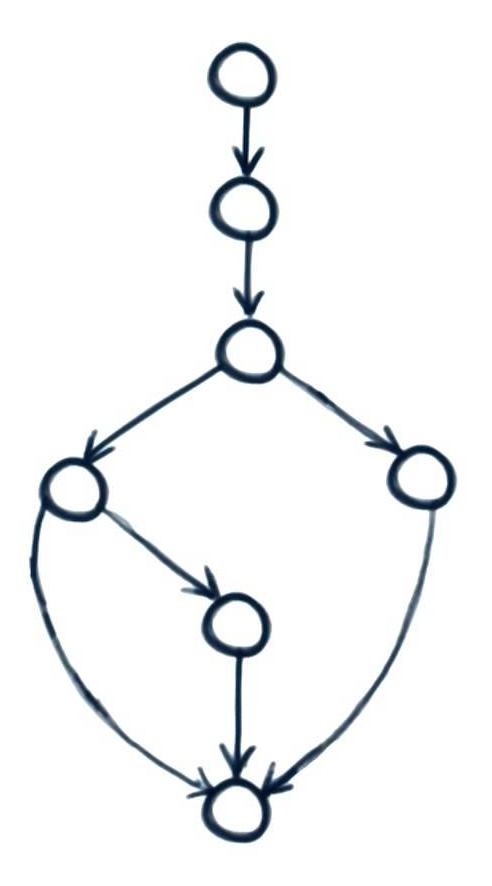
\includegraphics[scale=0.25]{controlflow}
	\end{textblock*}
	
	\begin{textblock*}{8cm}(4.5cm,3cm)
		\begin{itemize}
			\item Undertainting and overtainting are nearly \textbf{unavoidable}!
			\begin{itemize}
				\item \textbf{Time of detection} vs \textbf{Time of attack}
			\end{itemize}
			\item \textbf{Sanitization problem}
			\item Pure dynamic taint analysis considers \textbf{data flows}...
			\item<2-> ...but it ignores \textbf{control-flows}
			\begin{itemize}
				\item<2-> What about different security policies for different I/O channels?
					  \newline $\rightarrow$ \textbf{Static analysis}
			\end{itemize}
		\end{itemize}
	\end{textblock*}
\end{frame}